\documentclass[12pt]{article}

%================================================================================
% PREAMBLE
%================================================================================

%----- Page Layout & Fonts ------------------------------------------------------
\usepackage[utf8]{inputenc}       % Handle UTF-8 encoding
\usepackage[T1]{fontenc}          % Use modern font encodings
\usepackage{geometry}             % For setting page margins
\geometry{a4paper, margin=1in}     % Set A4 paper with 1-inch margins on all sides
\usepackage{lmodern}              % Use the Latin Modern font for a clean look
\usepackage{microtype}            % Improves typography and justification

%----- Math & Symbols -----------------------------------------------------------
\usepackage{amsmath}              % For advanced math environments

%----- Citations & Bibliography -------------------------------------------------
\usepackage[
    backend=biber,
    style=ieee,
    sorting=none
]{biblatex}
\addbibresource{references.bib}   % Specify the name of your .bib file
\usepackage{csquotes}             % For context-sensitive quotation marks with \enquote{}

%----- Hyperlinks ---------------------------------------------------------------
\usepackage{hyperref}
\hypersetup{
    colorlinks=true,
    linkcolor=blue,
    filecolor=magenta,      
    urlcolor=cyan,
    pdftitle={Coral Reef Monitoring with Computer Vision},
    pdfauthor={Your Name},
}

% Images
\usepackage{graphicx}
\usepackage{float}          % for [H] placement if you want it fixed
\graphicspath{{Result-figures/}}   % optional: where your images live

%================================================================================
% DOCUMENT START
%================================================================================
\begin{document}

\begin{titlepage}
\centering

% University / Course
{\Large Eindhoven University of Technology\par}
\vspace{6pt}
{\large Capstone Data Challenge (JBG060)\par}

\vspace{24pt}

% Title
{\LARGE\bfseries Coral-MTL: Hierarchical Multi-Task Learning for Coral Reef Health Assessment\par}

\vspace{18pt}

% (Optional) Subtitle line; you can remove this if you prefer
{\large Final Report\par}

\vspace{24pt}

% Authors (6 members). Replace with real names/IDs/emails.
\begin{minipage}{0.92\linewidth}
\centering
\begin{tabular}{l}
\textbf{Alessandro Da Ros} \quad \href{mailto:a.da.ros@student.tue.nl}{a.da.ros@student.tue.nl} \\
\textbf{Ergi Livanaj} \quad \href{mailto:e.livanaj@student.tue.nl}{e.livanaj@student.tue.nl} \\
\textbf{Sushrut Patil} \quad \href{mailto:s.patil@student.tue.nl}{s.patil@student.tue.nl} \\
\textbf{Alexandru Radu} \quad \href{mailto:i.a.radu@student.tue.nl}{i.a.radu@student.tue.nl} \\
\textbf{Gabriel Merle} \quad \href{mailto:g.merle@student.tue.nl}{g.merle@student.tue.nl} \\
\textbf{Mateusz Lotko} \quad \href{mailto:m.lotko@student.tue.nl}{m.lotko@student.tue.nl} \\
\end{tabular}
\end{minipage}

\vfill

% (Optional) Supervisor/Coach – uncomment and fill if needed
% {\small Supervisor: Dr.\ Firstname Lastname \quad|\quad Coach: Firstname Lastname, MSc\par}
% \vspace{6pt}

% Date
{\large \today\par}

\end{titlepage}

% ===================== BODY START =====================
\section{Context / Problem Background / Motivation of Analysis}

ReefSupport needs reef health intelligence at the same pace that images are collected. Right now, imagery arrives far faster than experts can annotate it. Managers then delay action or act on partial evidence. The stakeholder’s brief asks for an automated segmentation model that (i) identifies what coral is present (genus-level or equivalent groups), (ii) indicates the health state that matters for management (live, bleached, dead), (iii) works on messy field data with variable lighting, turbidity, motion blur and sensor differences, and (iv) is honest about uncertainty so scarce expert time can be routed to the hardest cases.

Manual workflows and semi-automated point counting improved throughput but still require human attention on every frame and miss colony boundaries \autocite{kohler2006cpce}. Early deep learning automated point classification but produced cover estimates from sparse samples \autocite{gonzalez2019seaview,gonzalez2020monitoring}. Dense, pixel-wise methods are now standard for scene understanding and better match the stakeholder’s needs, because cover, lesion tracking, and habitat mapping all depend on boundaries \autocite{xie2021segformer}. Our problem framing follows naturally: a unified, uncertainty-aware model that outputs both \emph{what} the coral is and \emph{how} it is doing, and that says when it is not confident.

\section{Business and Data Understanding}

\paragraph{Prior approaches and the gap.} There are three main families with clear trade-offs.  
1) \emph{Sparse point} methods scale cheaply but miss shapes and cannot track edges over time \autocite{kohler2006cpce,gonzalez2020monitoring}.  
2) \emph{Dense, class-agnostic} segmentation yields masks but does not jointly resolve taxonomy and health, so it cannot answer management’s “what and how” in one pass \autocite{zheng2024coralscop}.  
3) \emph{Health-only} systems detect bleaching but lack genus context that helps disambiguate look-alikes (for example, algae on rock versus algae on dead skeleton) \autocite{qin2025causal}.

The gap we address is an \emph{operational} framework for \emph{simultaneous dense genus and dense health} segmentation that (a) is robust to field variation and (b) exposes calibrated confidence for human triage \autocite{caruana1997,liu2019end,goncalves2023mtlsegformer}.

\paragraph{Data and relevance.} We use the Coralscapes dataset, a modern, densely annotated coral dataset with pixel-level labels for \textbf{39} benthic classes, including live, bleached, and dead states \autocite{sauder2025coralscapes}. The record contains \textbf{2075} images from \textbf{35} sites, spanning \textbf{5} countries bordering the Red Sea. Labels were produced under an expert protocol. This dual-label structure directly supports the two-head design in a single model. Diversity in depth, turbidity, and illumination aligns with our robustness goal. Beyond labels, we add physics-plausible augmentations (haze, color shift, blur) so training sees the conditions that cause failures in the field; these degradations are well documented in underwater vision \autocite{cong2024uieSurvey}. While stakeholder-provided datasets were considered, they were deferred from primary training as they lacked the concurrent morphology and health labels essential for our approach. This introduces a potential generalization gap, leaving domain-specific fine-tuning using their data as critical future work.

\paragraph{Framework introduction and background} Multi-Task Learning (MTL) is a paradigm where a single model concurrently solves multiple related tasks \autocite{kutvonen2020mtl}. This approach typically uses a shared network backbone to learn a common feature representation, from which multiple task-specific ``heads'' branch off to produce distinct outputs. This shared learning process functions as a form of implicit regularization, forcing the model to develop more robust and generalizable representations. This often leads to improved performance on all tasks compared to training separate, single-task models.

\section{Research Objective}

\textbf{Objective.} Train and evaluate a single model that jointly segments genus and health from underwater imagery, improves boundary quality over a strong baseline, and \emph{reports probability calibration (ECE, NLL, Brier) without post-hoc modification}, supporting expert review by exposing confidence and error patterns.

\paragraph{Assumptions and scope.} Evaluation is limited to this dataset; cross-region transfer is future work. We assume genus and health are complementary signals and that explicit information exchange can exploit that complementarity \autocite{liu2019end,goncalves2023mtlsegformer}. Because the target is field use, \emph{boundary quality} and \emph{calibration} are first-class objectives alongside mIoU \autocite{cheng2021boundaryiou,guo2017calibration}.

\paragraph{Success criteria.}  
1) \emph{Accuracy:} higher global mIoU and stronger boundary metrics (BIoU, Boundary F1) than the baseline \autocite{cheng2021boundaryiou}.  
2) \emph{Calibration:} Report ECE, NLL, and Brier for the trained models to characterize confidence quality.
3) \emph{Diagnostic Clarity:} Diagnostic error decomposition to identify model failure modes \autocite{bolya2020tide}.
4) \emph{Robustness:} performance holds under site hold-out and under stress augmentations (turbidity, blur, color cast) \autocite{cong2024uieSurvey}.  
5) \emph{Efficiency:} inference fits platform latency and memory constraints \autocite{xie2021segformer}.

\section{Approach}

\paragraph{Pipeline.} Images are tiled; we apply physics-plausible augmentations; a shared SegFormer-style encoder builds multi-scale features; two \emph{primary} decoders output genus and health; \emph{five lightweight auxiliary heads} (fish, human artifacts, substrate, background, biota) supply context; we export masks and probabilities for platform use \autocite{xie2021segformer,goncalves2023mtlsegformer}.

\paragraph{Information sharing.}
We adopt multi-task learning (MTL) with explicit feature exchange between the two primary heads (genus, health): morphology cues support health decisions and vice versa. Five lightweight context heads (fish, human artifacts, substrate, background, biota) regularize shared features and sharpen edges around corals. The overall architecture and the exact differences between the Baseline, MTL Focused, and MTL Holistic variants are summarized in Fig.~\ref{fig:arch-compare}. The cross-attention mechanism used for feature exchange between primary tasks is detailed in Fig.~\ref{fig:feature-exchange}.

\paragraph{Losses and optimization.} Both MTL variants in the reported results use \emph{IMGrad} to mitigate task imbalance by re-scaling gradients, improving stability, and allowing auxiliaries to help rather than dominate \autocite{zhou2025imgrad}. Base segmentation losses are \emph{Dice + focal} \autocite{milletari2016vnet,lin2017focal}. We monitor gradient norms and cosine similarity to detect conflict. IMGrad delivered stable training and strong early gains with minimal added complexity \autocite{yu2020pcgrad}.

\paragraph{Splits and leakage controls.} We use \emph{site-level hold-out} to simulate deployment, remove near-duplicate frames across splits, and separate temporally adjacent frames. \emph{Poisson-disk sampling} focuses training on information-rich tiles and reduces oversampling of near-identical patches \autocite{bridson2007poisson}. These controls reduce optimistic bias and make validation a better proxy for the platform’s future data.

\paragraph{Calibration (measured only).}
We quantify probabilistic calibration but do not modify model confidences post hoc. Specifically, we report Expected Calibration Error (ECE), Negative Log-Likelihood (NLL), and Brier score on the test set to characterize how well predicted probabilities correspond to empirical accuracy; we do not apply temperature scaling or any abstention policy.

\paragraph{Error Decomposition.} We use a TIDE-inspired error decomposition to diagnose failure modes beyond aggregate metrics. By categorizing errors into Classification, Background (False Positives), and Missed (False Negatives), we can pinpoint specific weaknesses (such as confusing similar genera or hallucinating corals) to guide targeted improvements \autocite{bolya2020tide}.

\paragraph{Deployment.} The model was deployed on a hosted High Performance Computing (HPC) virtual machine featuring a GPU with over 48GB of VRAM \footnote{The virtual machines in question were rented via a GPU provider service, namely \url{vast.ai}. A minimum of 48GB of VRAM is required.}. This powerful infrastructure was essential for executing our complete machine learning pipeline, from data-centric sampling and advanced MTL training to the comprehensive, resource-intensive evaluation protocol.

\section{Evaluation Methodology}

\paragraph{Quantitative.}
We evaluate global mIoU, per-class IoU, boundary-sensitive metrics (BIoU and Boundary~F1), and probability calibration (ECE, NLL, Brier). To complement IoU-based summaries, we analyze class-specific precision–recall (PR) curves and Average Precision (AP) for the top-3 frequent genus and health classes (Fig.~\ref{fig:pr-top3}); PR/AP capture threshold-swept behavior and are informative for rare classes. All calibration values reflect the model \emph{as trained} (no post-hoc calibration).

\paragraph{Model selection and statistics.}
Model selection prioritizes a combination of mIoU and boundary quality (BIoU, Boundary~F1). We report paired, image-level bootstrap intervals (95\%) for key deltas where relevant. Learning dynamics are shown per task in Fig.~\ref{fig:learning-curves}.

\paragraph{Qualitative and stress testing.}
We inspect representative scenes to verify that quantitative gains correspond to cleaner colony perimeters and fewer background false positives; visual comparisons for all three models appear in Figs.~\ref{fig:qual-baseline}-\ref{fig:qual-holistic}. In addition, we review error-type composition (classification, background FP, missed FN) in Fig.~\ref{fig:error-decomp}.

\section{Results}

\paragraph{Headline comparison.}
The \emph{MTL Holistic} model outperforms both the Baseline and MTL Focused on the main test metrics (Table~\ref{tab:app-global}). The largest gains are boundary-sensitive: BIoU and Boundary~F1 increase most for Holistic, consistent with cleaner colony perimeters needed for cover estimation and lesion tracking. Training dynamics by task show faster early gains and a higher plateau for Holistic (Fig.~\ref{fig:learning-curves}).

\paragraph{Per-class and task patterns.}
Grouped per-class IoU bars for the most frequent genus and health categories are shown in Fig.~\ref{fig:per-class-bars}. Improvements are broad but not uniform: Holistic leads on many classes while the Baseline remains competitive on a few high-frequency categories. The Pareto-style view in Fig.~\ref{fig:pareto} summarizes the joint trade-off between genus and health (grouped), where Holistic achieves the best combined performance.

\paragraph{Precision-recall behavior.}
PR curves for the top-3 genus and health classes (Fig.~\ref{fig:pr-top3}) show near-saturated AP for common genera (e.g., \emph{massive/meandering}, \emph{pocillopora}). Health classes are more nuanced: for \emph{dead coral}, MTL Focused maintains higher precision at low recall, while \emph{bleached coral} exhibits a different ranking in PR space than in IoU, illustrating the known tension between threshold-swept PR and thresholded IoU summaries. This reinforces the need to view IoU and PR jointly when judging class-specific performance.

\paragraph{Error decomposition.}
Relative to the Baseline, both MTL variants reduce classification errors and background false positives; Holistic is the most conservative and shows the largest drop in background FP alongside an increase in missed regions (Fig.~\ref{fig:error-decomp}). This matches the boundary gains observed elsewhere and suggests more precise but tighter masks in difficult, low-contrast areas.

\paragraph{Qualitative outcomes.}
Visual comparisons (Figs.~\ref{fig:qual-baseline}-\ref{fig:qual-holistic}) confirm the quantitative patterns: Holistic produces smoother, crisper edges and fewer background activations around coral-shaped substrate, while some fine structures remain under-segmented in the hardest scenes.

\section{Discussion}

\paragraph{Why the approach helps boundaries.}
Context heads (fish, human artifacts, substrate, background, biota) reduce “coral-shaped background” confusions; explicit feature exchange between genus and health further sharpens edges by sharing morphology and appearance cues. Together, this yields the largest relative gains in boundary metrics (Table~\ref{tab:app-global}) and cleaner perimeters in the qualitative panels (Figs.~\ref{fig:qual-baseline}-\ref{fig:qual-holistic}).

\paragraph{Trade-offs and fixes.}
The conservative behavior that reduces false positives can increase missed regions. Two levers are most effective: (1) \emph{loss rebalancing} - tuning focal parameters and class weights for faint or bleached categories to recover recall without eroding boundaries; and (2) \emph{targeted data} - augmentation schedules and small curated additions (low-contrast, high-turbidity scenes) to increase sensitivity where the model under-segments.

\paragraph{Calibration stance.}
We report calibration (ECE, NLL, Brier) as measured; we do not apply post-hoc calibration or confidence-based abstention in this study. Future work will examine lightweight post-hoc calibration and threshold policies, but those are out of scope for the present results.

\paragraph{Robustness and monitoring.}
We evaluate robustness using site-level hold-out splits that mimic deployment to new locations, and we stress the models qualitatively on low-contrast scenes and turbid water. Improvements from the MTL variants persist under these conditions, though very low contrast remains challenging. For operational monitoring, we propose simple drift checks (summary color statistics, class-frequency ratios) and periodic spot audits on a small, freshly annotated sample. If drift is detected, we fine-tune on a compact buffer from the new conditions and re-run the same test protocol. We track boundary-sensitive metrics alongside mIoU because perimeters drive cover estimates and change detection (see Table~\ref{tab:app-global} and Figs.~\ref{fig:learning-curves}, \ref{fig:qual-baseline}-\ref{fig:qual-holistic}).

\paragraph{Objective fulfillment.}
The system meets the stated objectives: it improves accuracy and boundary quality over the baseline, jointly segments genus and health, and reports calibration as measured, without modifying confidences. Remaining weaknesses are concentrated in very low-contrast regions and a few frequent classes; the analysis above identifies concrete levers (loss rebalancing, targeted data) to address them. The model is ready for platform integration with the evaluation and monitoring steps described here.

\paragraph{Limits and future work.}
This study is constrained to one dataset; cross-region validation and camera-domain generalization are planned. For the modeling aspect, we recommend exploring class-aware thresholds, small curated data additions for faint/bleached categories, and lightweight post-hoc calibration methods as optional deployment toggles. Active learning that selects scenes using error-type signals and class coverage could also be worth testing, which aims to reduce annotation cost while improving recall where the models currently under-segment.

\section{Conclusion}

We deliver a unified multi-task segmentation model that improves global mIoU and boundary quality over a strong SegFormer baseline. The \emph{Holistic MTL} variant achieves the largest gains, cleaner colony perimeters (higher BIoU/Boundary~F1), broader per-class improvements, and more stable learning, matching operational needs for cover estimation and change detection \autocite{xie2021segformer,cheng2021boundaryiou}. For deployment, we recommend targeted augmentation or light fine-tuning for the frequent classes where the baseline still leads. Testing with other datasets is highly recommended as well. Together, these choices turn dense predictions into practical, trustworthy summaries for ReefSupport’s Open Coral AI.

% ===================== BODY END =====================

%TC:ignore
% ===================== APPENDIX =====================
\clearpage
\appendix
\renewcommand{\thefigure}{\arabic{figure}}
\renewcommand{\thetable}{\arabic{table}}
\setcounter{figure}{0}
\setcounter{table}{0}

\section*{Appendix}
\addcontentsline{toc}{section}{Appendix}

% ---------- Table 1: Global metrics ----------
\begin{table}[!htbp]
  \centering
  \caption{Test metrics (higher is better except NLL, ECE, Brier).}
  \label{tab:app-global}
  \begin{tabular}{lccc}
    \hline
    Metric & Baseline & MTL Focused & MTL Holistic \\
    \hline
    Global mIoU      & 0.3888 & 0.4039 & \textbf{0.4272} \\
    Global BIoU      & 0.0937 & 0.1075 & \textbf{0.1243} \\
    Boundary F1      & 0.1714 & 0.1942 & \textbf{0.2211} \\
    NLL $\downarrow$ & \textbf{1.2239} & 1.3995 & 1.5162 \\
    ECE $\downarrow$ & \textbf{0.1014} & 0.1275 & 0.1423 \\
    Brier $\downarrow$ & 0.5016 & 0.4959 & \textbf{0.4937} \\
    \hline
  \end{tabular}
\end{table}

% ---------- Figure A1: Architecture overview ----------
\begin{figure}[!htbp]
  \centering
  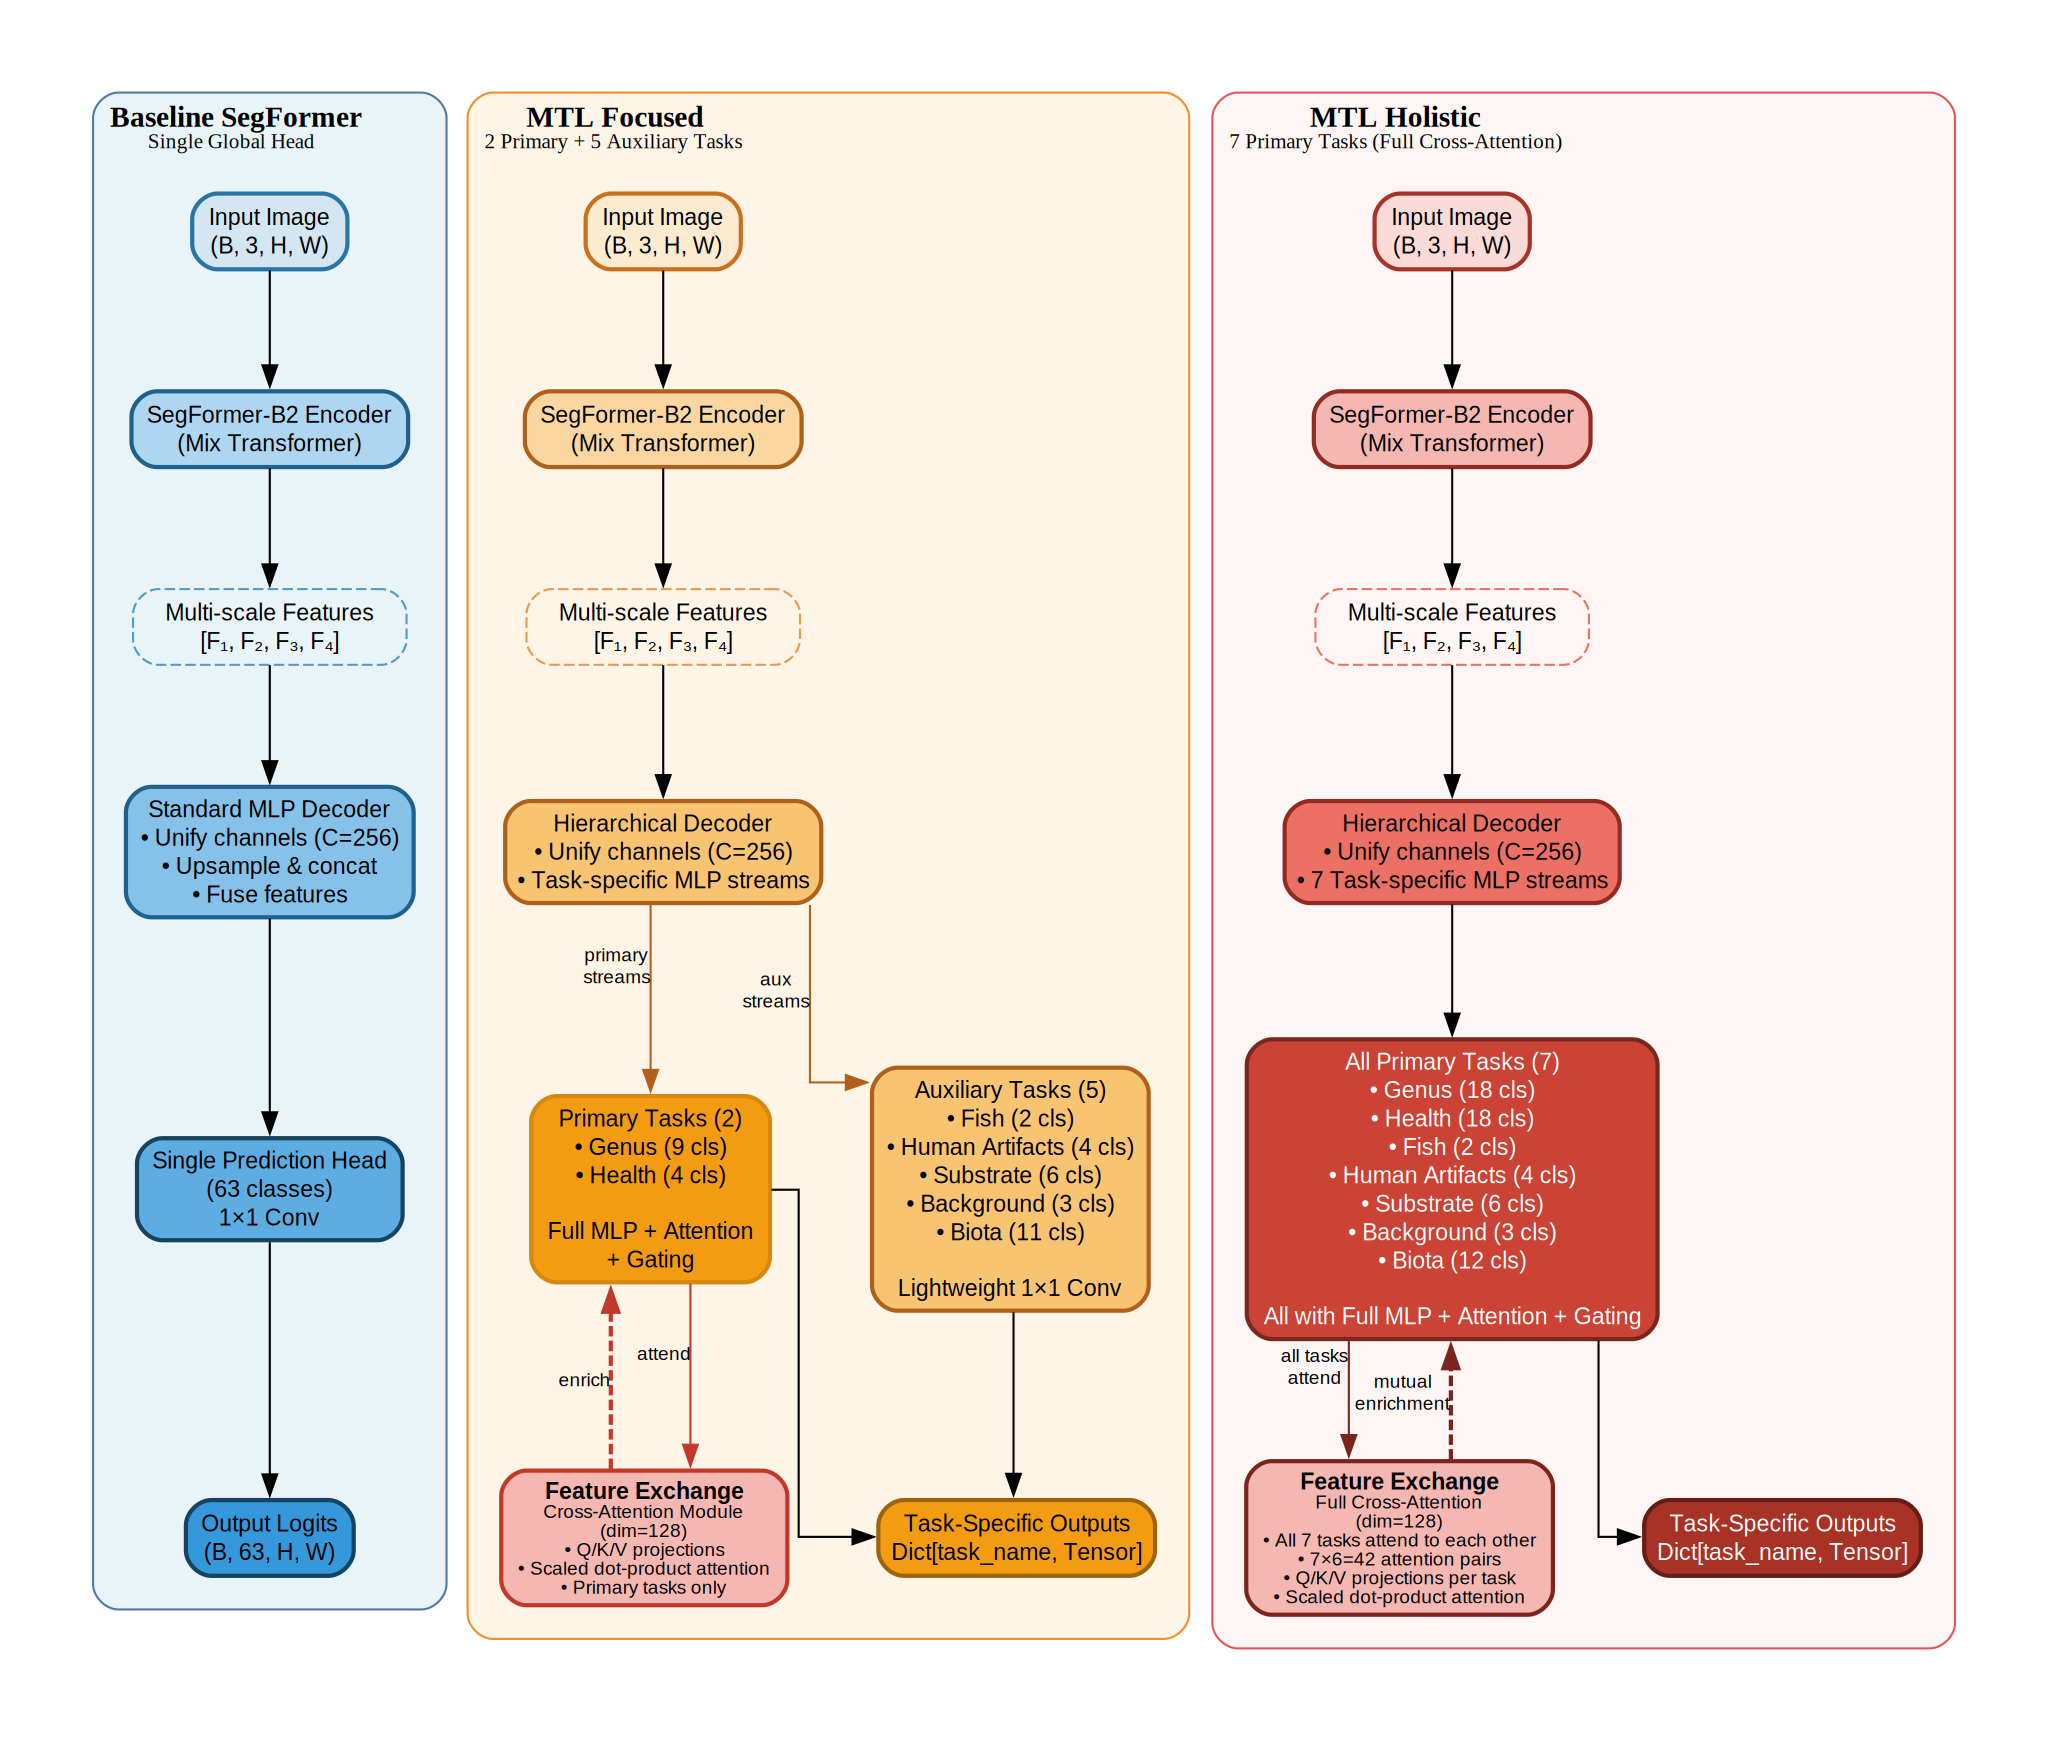
\includegraphics[width=\linewidth,keepaspectratio]{architecture_comparison.png}
  \caption{Architectural overview and comparison: Baseline, MTL Focused, and MTL Holistic.}
  \label{fig:arch-compare}
\end{figure}

% ---------- Figure A2: Feature exchange detail ----------
\begin{figure}[!htbp]
  \centering
  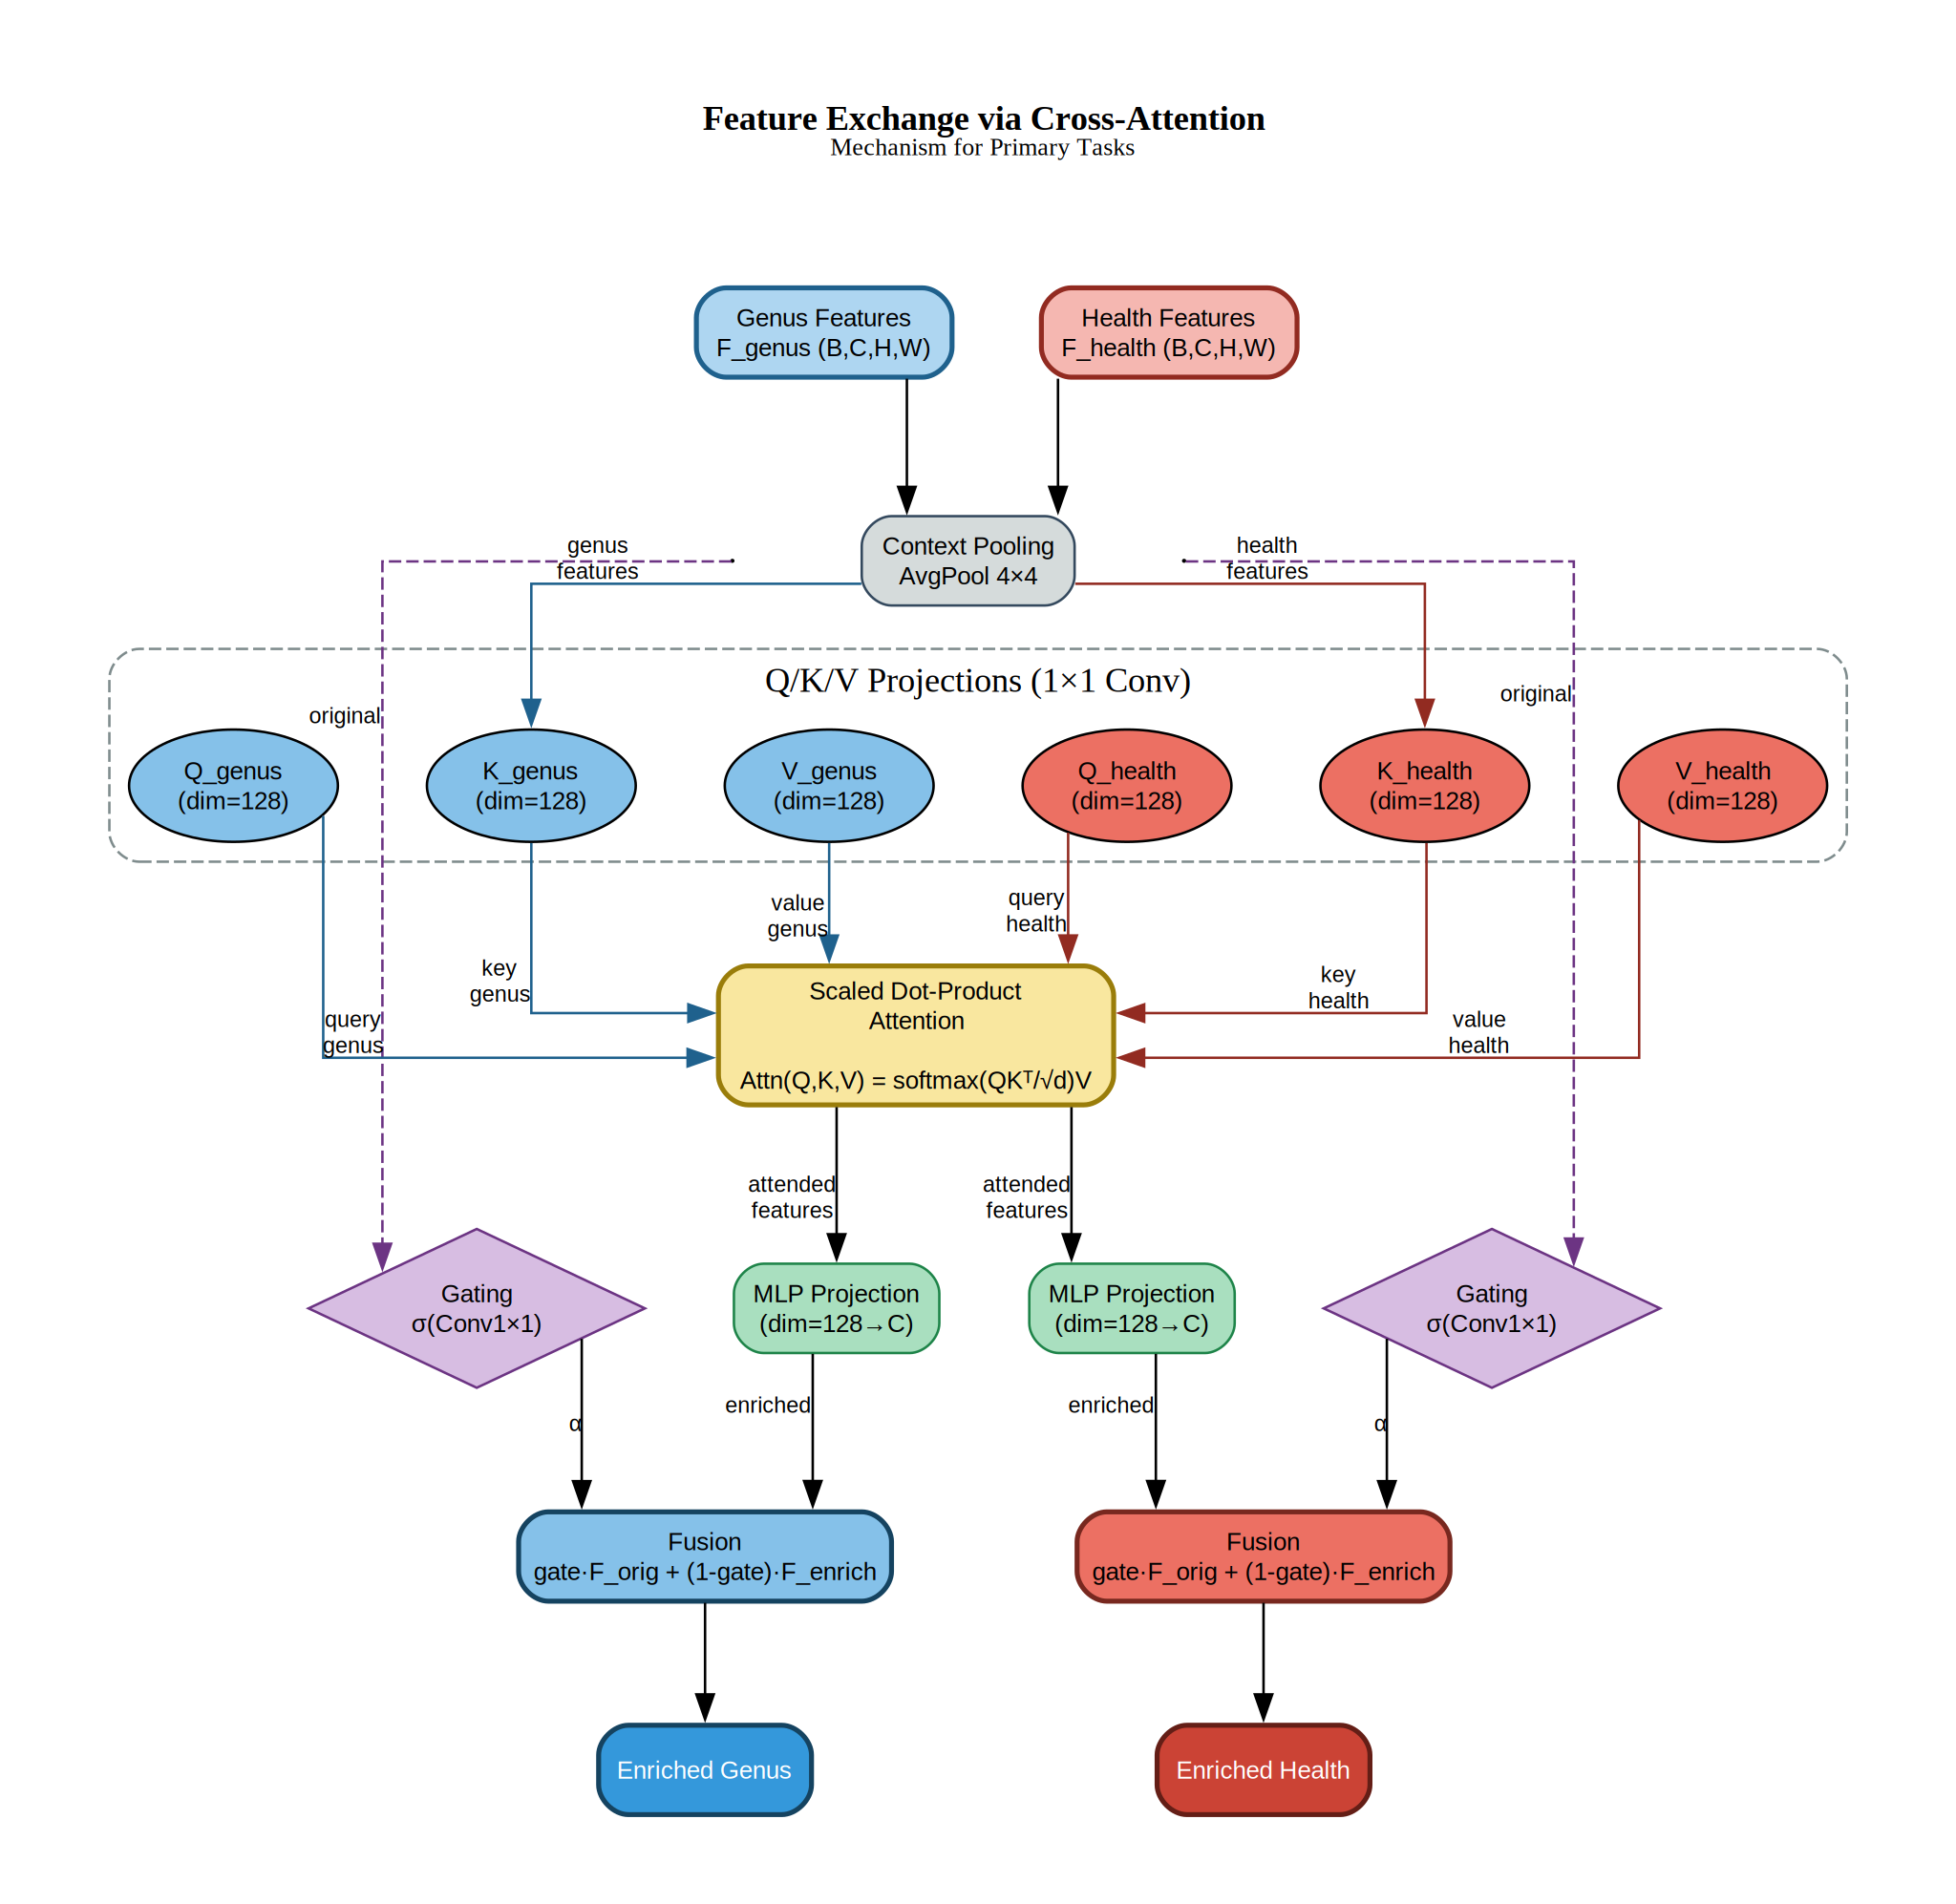
\includegraphics[width=\linewidth,keepaspectratio]{feature_exchange_detail.png}
  \caption{Feature exchange via cross-attention between the two primary tasks (genus, health).}
  \label{fig:feature-exchange}
\end{figure}

% ---------- Figure A3: Per-task learning curves ----------
\begin{figure}[!htbp]
  \centering
  \includegraphics[width=\linewidth,keepaspectratio]{per_task_learning_curves.png}
  \caption{Per-task learning curves for genus and health: mIoU and BIoU across epochs.}
  \label{fig:learning-curves}
\end{figure}

% ---------- Figure A4: Per-class IoU bars ----------
\begin{figure}[!htbp]
  \centering
  \includegraphics[width=\linewidth,keepaspectratio]{per_class_iou_bars.png}
  \caption{Grouped per-class IoU comparison for top genus and health categories.}
  \label{fig:per-class-bars}
\end{figure}

% ---------- Figure A5: Genus–health Pareto ----------
\begin{figure}[!htbp]
  \centering
  \includegraphics[width=0.7\linewidth,keepaspectratio]{pareto_genus_health.png}
  \caption{Genus vs health trade-off (grouped mIoU) across models.}
  \label{fig:pareto}
\end{figure}

% ---------- Figure A6: Precision–recall ----------
\begin{figure}[!htbp]
  \centering
  \includegraphics[width=\linewidth,keepaspectratio]{pr_curves_top3.png}
  \caption{Precision–recall curves for the top-3 genus and health classes (excluding unlabeled).}
  \label{fig:pr-top3}
\end{figure}

% ---------- Figure A7: Error decomposition (kept) ----------
\begin{figure}[!htbp]
  \centering
  \includegraphics[width=\linewidth,keepaspectratio]{error_decomposition_3models.png}
  \caption{Error decomposition across models: classification, background FP, and missed FN.}
  \label{fig:error-decomp}
\end{figure}

% ---------- Figure A8–A10: Qualitative panels ----------
\begin{figure}[!htbp]
  \centering
  \includegraphics[width=\linewidth,keepaspectratio]{qual_baseline_combined.png}
  \caption{Baseline SegFormer: RGB, ground truth, predictions, and error maps (genus/health).}
  \label{fig:qual-baseline}
\end{figure}

\begin{figure}[!htbp]
  \centering
  \includegraphics[width=\linewidth,keepaspectratio]{qual_mtl_focused_combined.png}
  \caption{MTL Focused: RGB, ground truth, predictions, and error maps (genus/health).}
  \label{fig:qual-focused}
\end{figure}

\begin{figure}[!htbp]
  \centering
  \includegraphics[width=\linewidth,keepaspectratio]{qual_mtl_holistic_combined.png}
  \caption{MTL Holistic: RGB, ground truth, predictions, and error maps (genus/health).}
  \label{fig:qual-holistic}
\end{figure}

% =================== END APPENDIX ====================

\clearpage
\printbibliography
%TC:endignore
\end{document}
